\section{Methods}

\subsection{Hardware}\label{subsection:A}
This section contains all hardware used in this capstone project.
    \subsubsection{Drone Kit}\label{subsection:A1}
    \begin{itemize}
        \item QWinOut Q705 6-Aixs RC Drone
        \item QWinOut J630 4-Aixs RC Drone
    \end{itemize}

    \begin{figure}[H]
        \centerline{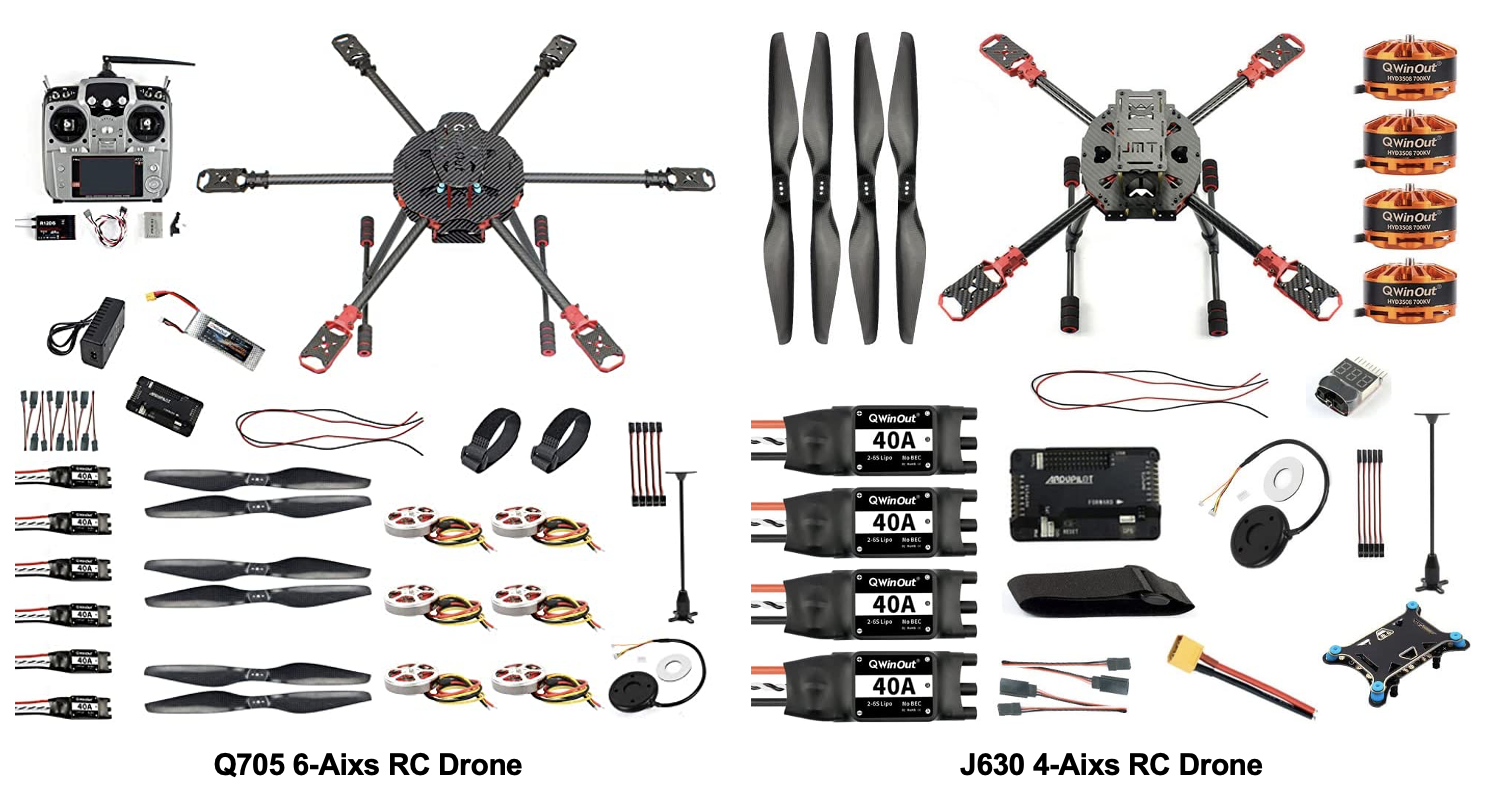
\includegraphics[width=0.5\textwidth]{Figures/Methods/Drone_Kits.png}}
        \caption{(left) 6-Axis RC Drone / (right) 4-Axis RC Drone.}
        \label{fig1}
    \end{figure}
    
    There are two types of drones used in the project, as shown in Fig.~\ref{fig1}, the larger 6-axis RC drone and the new smaller 4-axis drone purchased this 2023 spring semester. The larger 6-axis drone is a continuation of the team's work from last semester, and the smaller 4-axis drone is a new drone that we assembled this semester.
    
    \subsubsection{Transistor \& Receiver}\label{subsection:A2}
    \begin{itemize}
        \item SIK Telemetry Radio
        \item Flysky FS-i6   6CH 2.4GHz RC Transmitter
        \item Flysky FS-i6X 10CH 2.4GHz RC Transmitter
        \item iA6B Receiver
        \item iA10B Receiver
    \end{itemize}

    \begin{figure}[H]
        \centerline{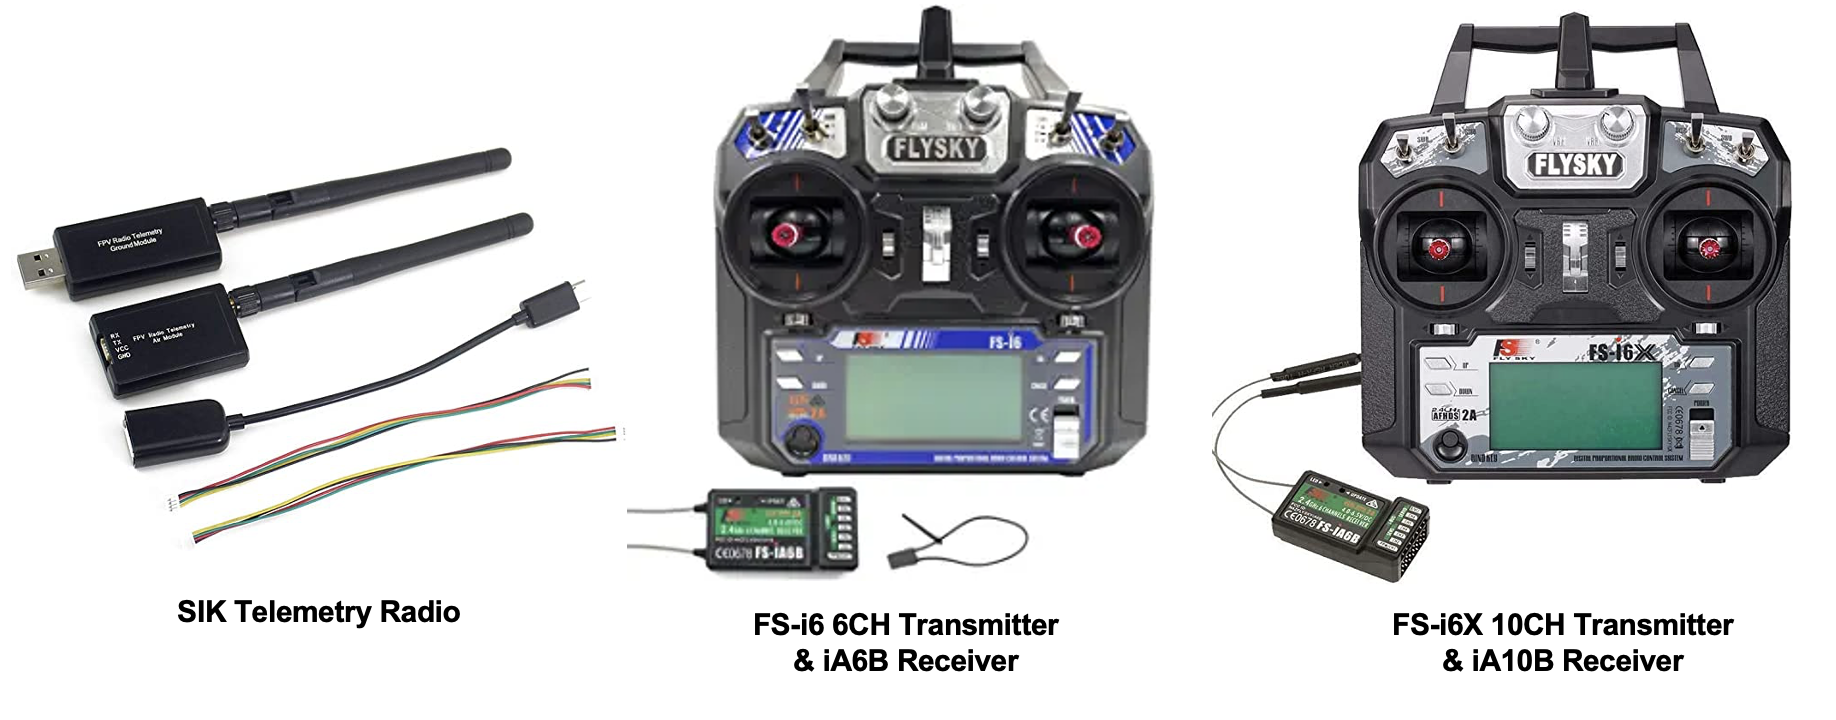
\includegraphics[width=0.5\textwidth]{Figures/Methods/Transistors&Receivers.png}}
        \caption{(left) SIK Telemetry Radio / (middle) FS-i6 6CH Transmitter \& iA6B Receiver / (right) FS-i6X 10CH Transmitter \& iA10B Receiver.}
        \label{fig2}
    \end{figure}

    Since we use two types of drones, there are different Transistors \& Receivers for each, as shown in Fig.~\ref{fig2}. FS-i6 6CH and iA6B Receiver pairing is for 6-axis drone. FS-i6X 10CH and iA10B Receiver pairing is for 4-axis drone. Then SIK radio just used to communicate between flight controller and Laptop/PC.
    
    \subsubsection{Flight Controller}\label{subsection:A3}
    \begin{itemize}
        \item Cube Black Flight Controller
        \item APM2.8 Flight Controller
    \end{itemize}

    \begin{figure}[H]
        \centerline{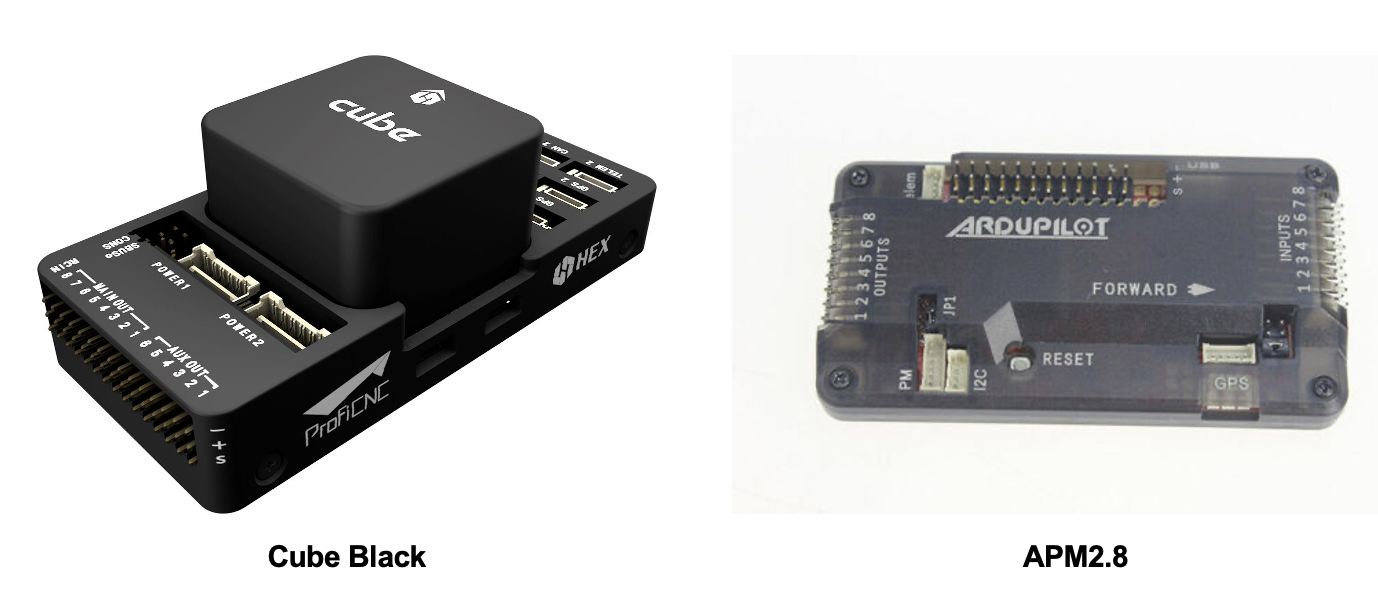
\includegraphics[width=0.5\textwidth]{Figures/Methods/Flight_Controllers.png}}
        \caption{(left) Cube Black / (right) APM2.8.}
        \label{fig3}
    \end{figure}

    Flight controller plays one of the crucial roles in this project, as it is responsible for controlling the drone's flight and stability. It receives sensor data from various sensors and makes necessary adjustments to maintain the desired altitude, orientation, and movement of the drone. It's including an accelerometer, gyroscope, magnetometer, and barometer.

    We used two flight controller modules that came with the Drone Kit in this project, as shown in Fig.~\ref{fig3}, so that we could expedite our development and spend more time on Deep Learning algorithms.
    
    \subsubsection{Embedded System / Controller}\label{subsection:A4}
    \begin{itemize}
        \item Jetson Nano 2GB
        \item Raspberry Pi 3B
        \item Raspberry Pi 4B
    \end{itemize}

     \begin{figure}[H]
        \centerline{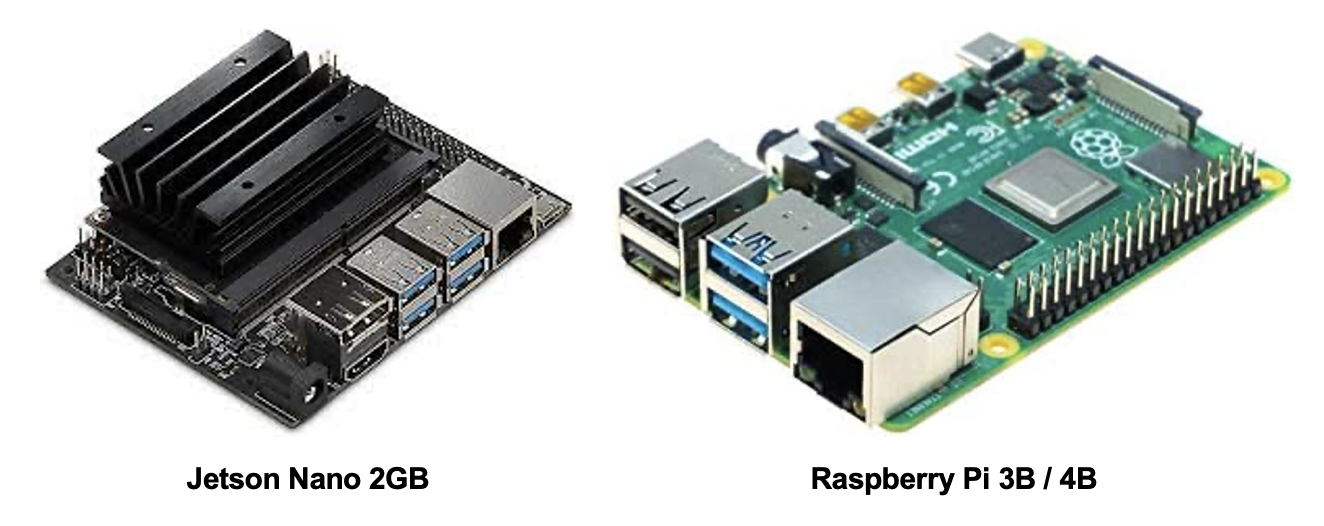
\includegraphics[width=0.5\textwidth]{Figures/Methods/Embedded_Systems.png}}
        \caption{(left) Jetson Nano 2GB / (right) Raspberry Pi 3B / 4B.}
        \label{fig4}
    \end{figure}

    The embedded system is the main controller in the system, which plays a critical role in performing all the tasks. It collects images from the camera sensor and uses deep learning algorithms to correctly identify flower types, track flower locations and calculate depth information, and then sends commands to the flight controller to precisely control the drone to successfully complete the artificial pollination task.

    Here we use two types of embedded devices, as shown in Fig.~\ref{fig4}, the Jetson Nano 2GB with built-in GPU and the smaller Raspberry Pi 3B / 4B. We will test these two types of embedded devices and compare which one is more compatible for the project.

\subsection{System Design}\label{subsection:B}

The system consists of essential components, including a Jetson Nano 2GB and/or Raspberry Pi to process deep learning models. The Drone-Kit API and MAVLink protocol facilitate communication with the Cube Black flight controller, which ultimately controls the drone's motor and navigation. The system flow chart is depicted in Fig.~\ref{fig5}.

Two embedded devices, the Jetson Nano and Raspberry Pi, are incorporated into the drone to compare their performance. Additionally, a SIK radio block is utilized to send the drone's status back to a Laptop/PC for real-time monitoring. For added safety, a Flysky FS-i6 6CH 2.4GHz RC Transmitter and iA6B Receiver are included to enable manual drone control.

    \begin{figure}[H]
        \centerline{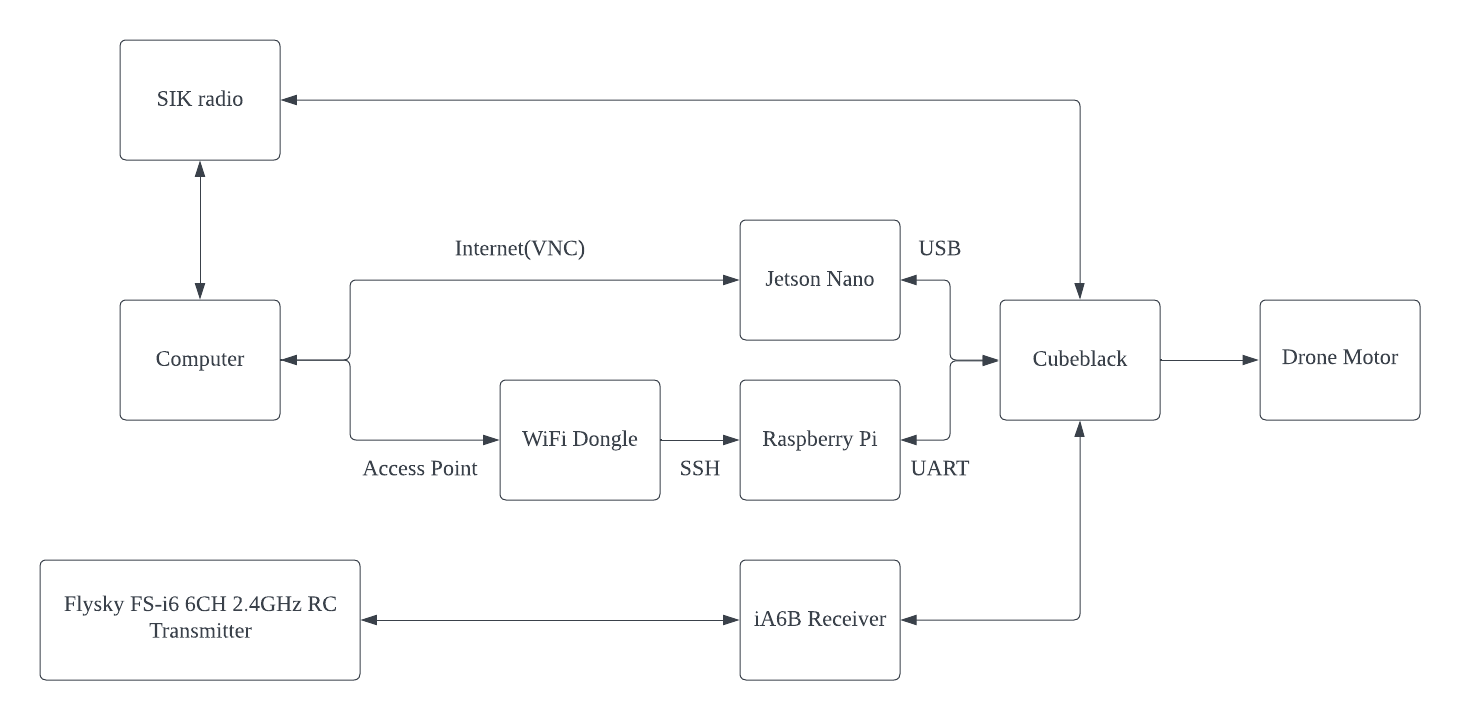
\includegraphics[width=0.5\textwidth]{Figures/Methods/System Flow Chart.png}}
        \caption{System Flow Chart.}
        \label{fig5}
    \end{figure}

    \begin{figure}[H]
        \centerline{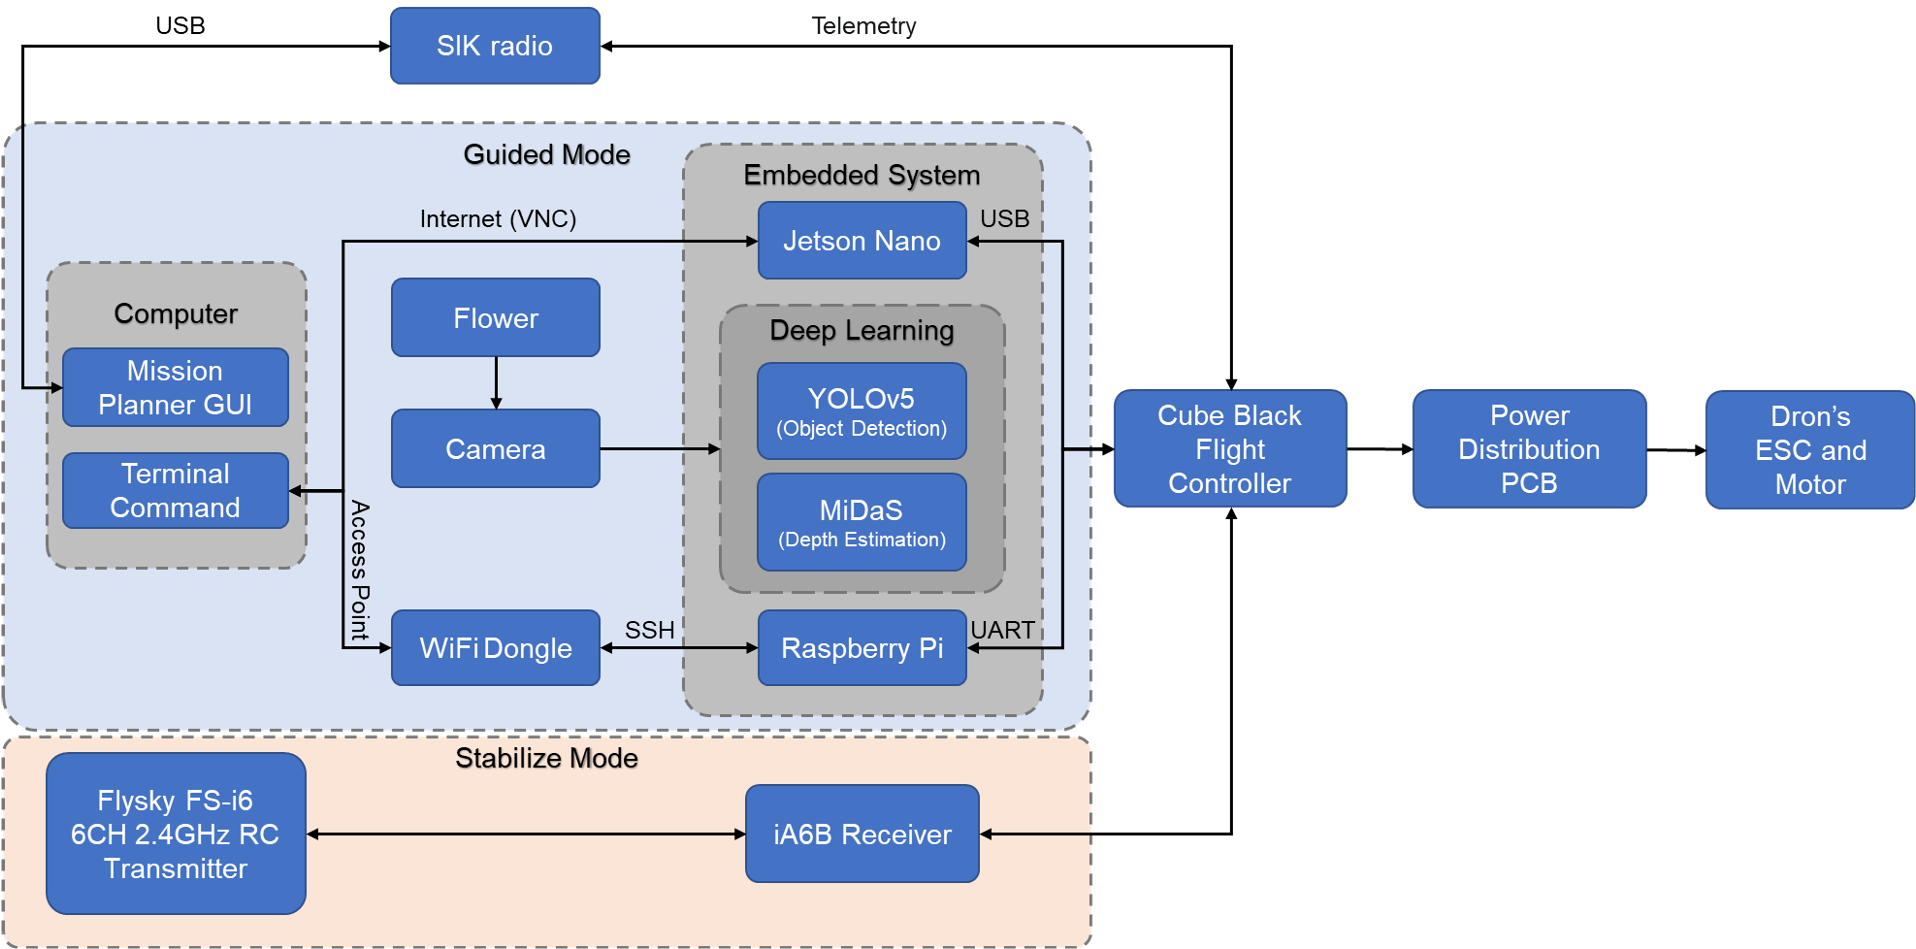
\includegraphics[width=0.5\textwidth]{Figures/Methods/System_Overall_Design.png}}
        \caption{Overall System Design.}
        \label{fig6}
    \end{figure}

Fig.~\ref{fig6} provides a detailed overview of the system design. The process starts with capturing an image of a flower using a camera sensor. The image is then analyzed using Deep Learning's YOLOv5 object detection model and MiDaS depth estimation model, both of which run on the Embedded System Jetson Nano 2GB and/or Raspberry Pi. YOLOv5 is used to detect flowers in the image (Please note sections \ref{subsection:C} below for more information on YOLOv5), while MiDaS calculates the distance between the flowers and the drone. (Please note sections \ref{subsection:D} below for more information on MiDaS)

 For manual control, we use the Flysky FS-i6 6CH 2.4GHz RC Transmitter in Stabilize Mode, which disables pre-arming checking and puts the drone in an unstable mode. However, to operate the drone using scripts, it must be set to Guided Mode, which allows pre-arming checks to ensure the drone is in a safe condition to complete the pollination task.
    
\subsection{YOLOv5}\label{subsection:C}

Object detection is a crucial aspect of autonomous drone operation. While there are many deep learning models that can be used for flower detection, Convolutional Neural Networks (CNNs) are the most researched method \cite{b5, b6}. However, these models mostly use a two-stage pipeline which may not be efficient for autonomous drone purposes. In contrast, one-stage models such as YOLO (You Only Look Once) \cite{b7} model is a state-of-the-art real-time object detection algorithm, known for its high speed and accuracy. YOLO processes the input image by dividing it into a grid and predicting a set of bounding boxes, objectness scores, and class probabilities for each grid cell. These predictions are combined and subjected to non-maximum suppression to remove overlapping boxes, generating the final object detections.

In our autonomous drone pollination project, the primary objective is to detect flowers using a webcam mounted on the drone. The YOLO model plays a crucial role in identifying flowers within the camera frame. We utilized the YOLOv5 architecture \cite{b8} for this project, which is an enhanced version of the original YOLO model. YOLOv5 is implemented in the PyTorch framework and offers a range of pre-trained models, each with different trade-offs between speed and accuracy. Given the limited computational resources available on drones, we chose the smaller YOLOv5 model, YOLOv5s, which has only 7.2 million parameters.

In addition to the model trained by the Ultralytics team, we also investigated the methods employed by the previous Autodrone team. They incorporated knowledge distillation \cite{b9} into the original YOLOv5 training framework, a technique that transfers knowledge from a larger model to a smaller model, thereby enhancing the performance of the smaller model. A larger model served as a teacher model, with its output functioning as a soft label to instruct the student model.

By leveraging the efficient YOLOv5s architecture and incorporating knowledge distillation, our flower detection model achieves high accuracy while maintaining real-time performance, making it suitable for deployment on resource-constrained platforms such as drones. This combination of techniques enables the autonomous drone pollination system to effectively detect flowers or other objects in real-world environments, thus constructing a key foundation for the autonomous pollination system.

\subsection{MiDaS}\label{subsection:D}

To accurately estimate the distance of flowers from the drone, we employed the MiDaS (Monocular Depth Estimation of High Resolution Images with Pyramid Stereo Fusion) model \cite{b10}. The MiDaS model is a state-of-the-art depth estimation algorithm known for its speed and accuracy. It can estimate depth from a single image without the need for stereo cameras. The model utilizes a deep neural network to learn a mapping between the input image and its corresponding depth map, which is subsequently used to calculate the distance of the flower from the drone.

While there are alternative methods to determine the distance between objects and the camera with higher accuracy, such as stereo vision, these approaches tend to consume more computing resources and power. Given the constraints of the embedded system on the drone, we opted to use the MiDaS depth estimation model based on a monocular camera. Theoretically speaking, this model allows us to estimate the depth of the flower using a single image captured by the drone, reducing computational requirements and power consumption while still providing reliable depth estimation.

The MiDaS depth map estimates the depth of each pixel in an input image, representing the distance of that pixel from the camera. However, several factors can affect the accuracy of the depth map, including the quality of the input image, the distance of the object from the camera, and the lighting conditions. To evaluate the performance of the MiDaS model and assess its suitability for depth estimation on a drone, we conducted two experiments aimed at determining the numerical relationship between the depth map intensity and the real-world distance in meters.

The first experiment was set up inside the ECE lab, as illustrated in Fig. ~\ref{fig7}. Multiple tapes were placed on the floor at 1-meter intervals. The camera was positioned steadily at the 0-meter line. In this controlled environment, chairs were placed on the marked lines and served as detected objects.

\begin{figure}[H]
    \centerline{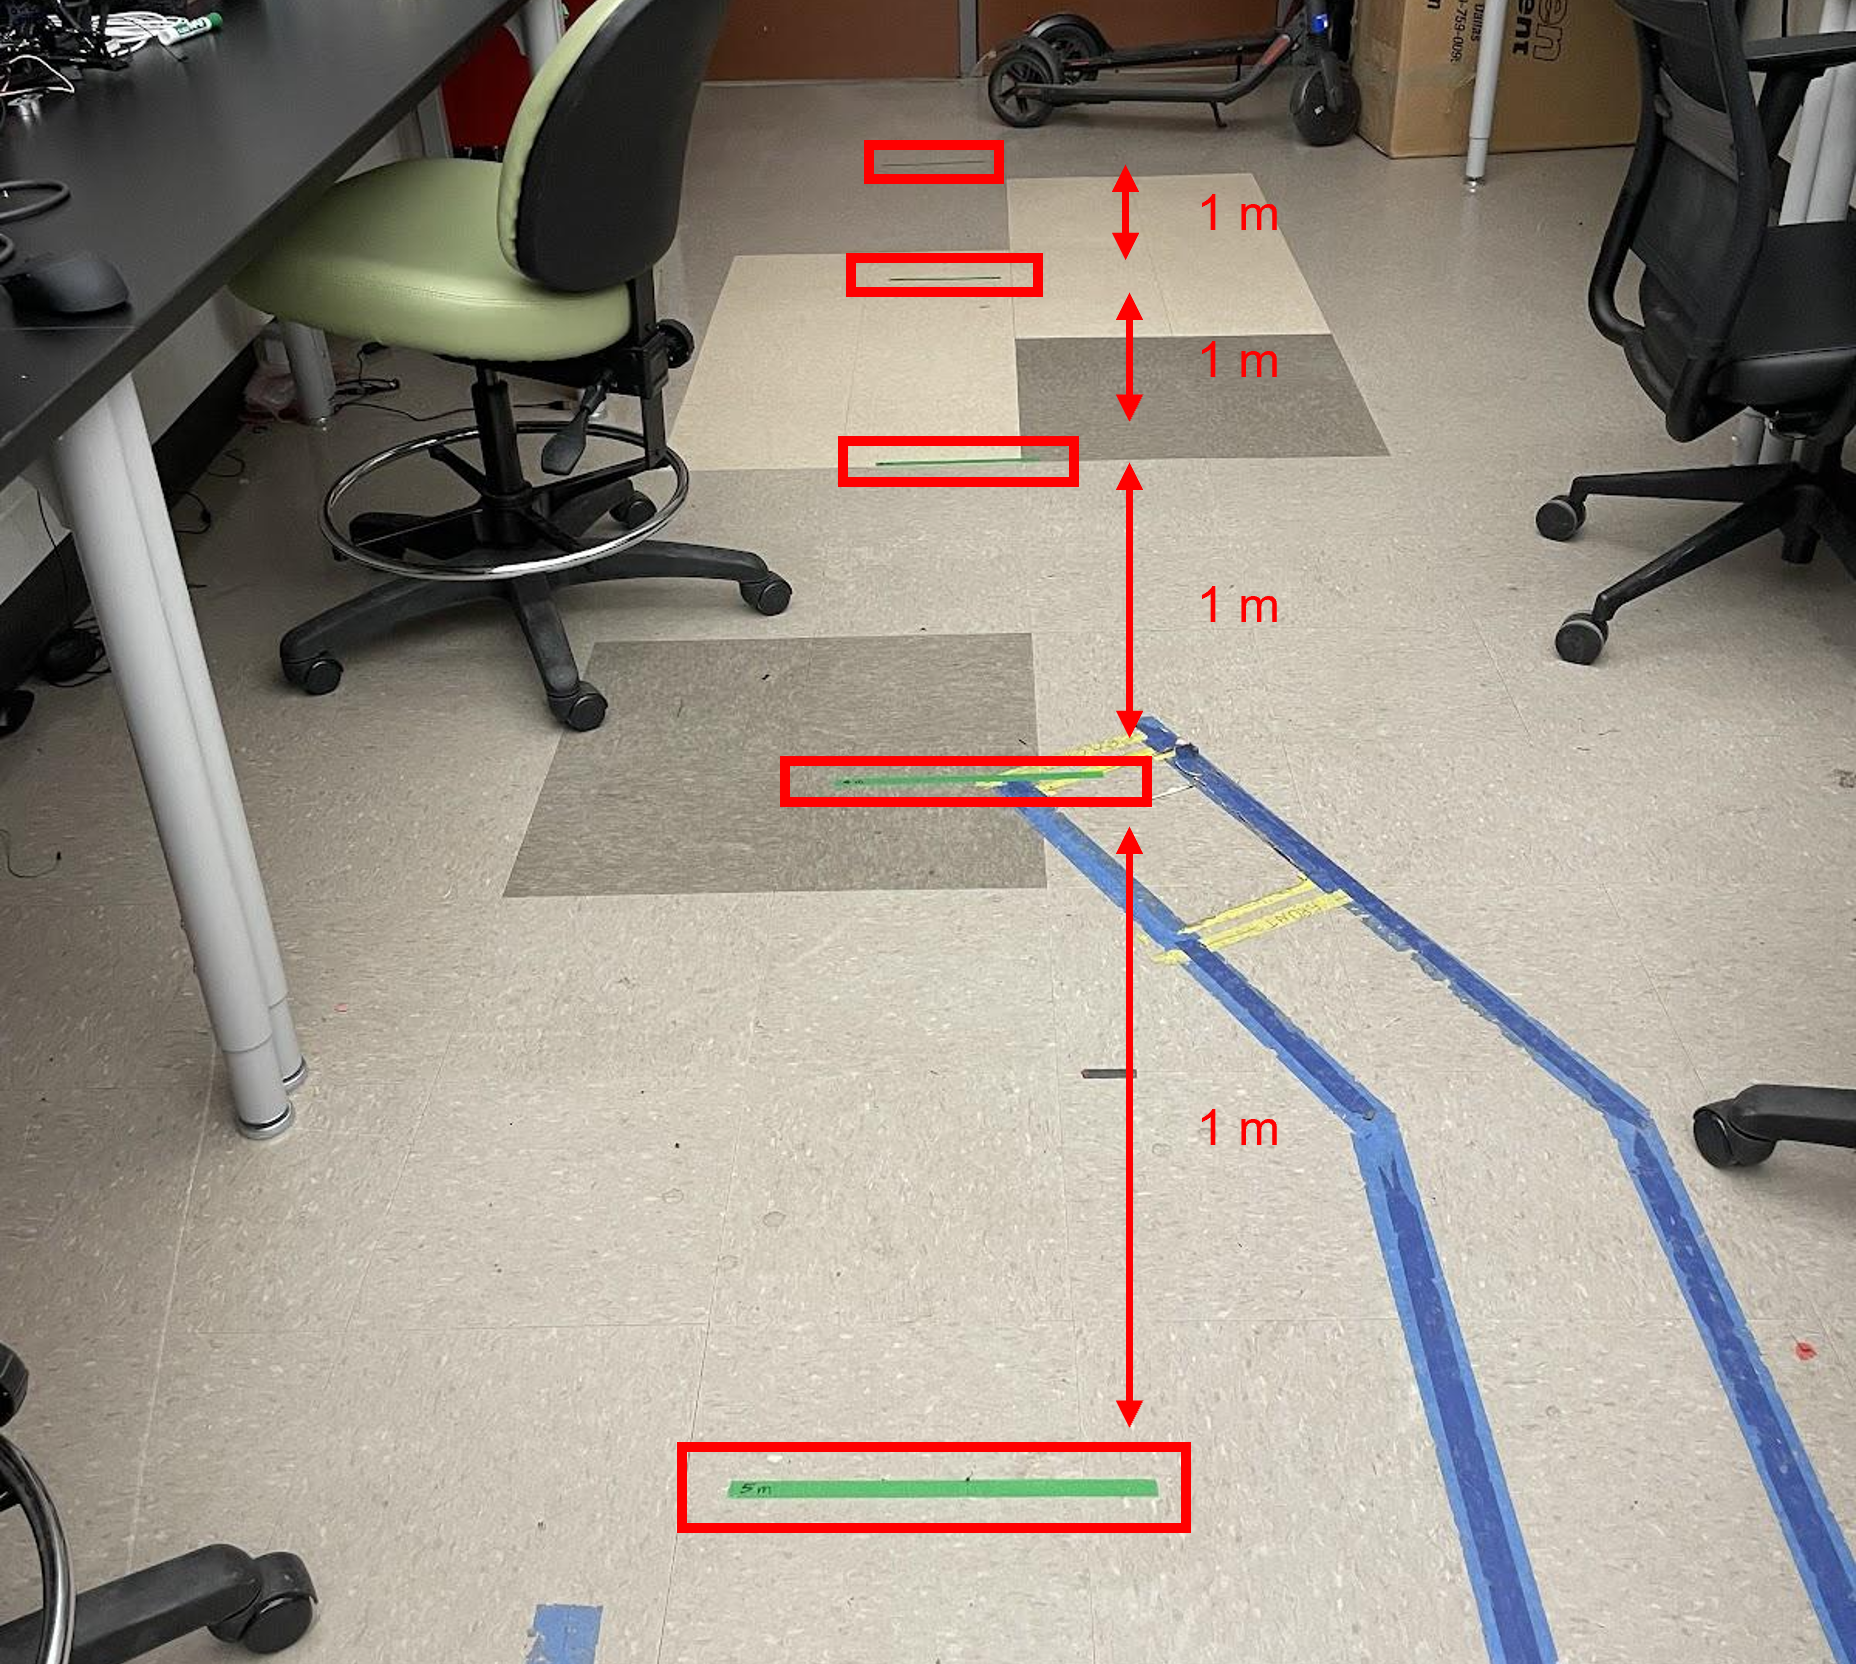
\includegraphics[width=0.5\textwidth]{Figures/Methods/env1.png}}
    \caption{Indoor Environment of the First Experiment}
    \label{fig7}
\end{figure}

    
The second experiment was conducted outdoors in an open environment, as shown in Fig. ~\ref{fig8.1}. The objective was to simulate object detection and depth estimation in a real autonomous pollination task with noise and unexpected anomalies occurring in the camera frame within a dynamic environment. The experiment involved a webcam mounted onto the drone, a team member carrying the drone and holding one end of a tape measure, and another team member holding the other end of the tape measure, acting as the detected object, and recording the actual distances from the camera. This experiment was performed twice from two different orientations to test whether the orientation of sunlight was another contributing factor to the depth map intensity.


\begin{figure}[H]
    \centerline{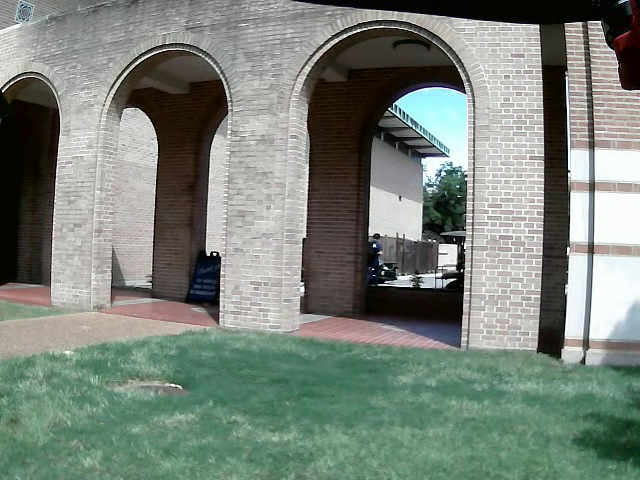
\includegraphics[width=0.5\textwidth]{Figures/Methods/env2a.png}}
    \label{fig8.1}
\end{figure}

\begin{figure}[H]
    \centerline{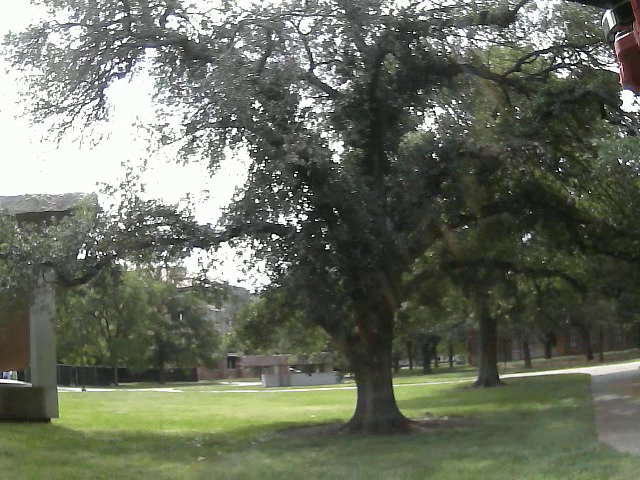
\includegraphics[width=0.5\textwidth]{Figures/Methods/env2b.png}}
    \caption{Outdoor Environments of the Second Experiment}
    \label{fig8.2}
\end{figure}

The results and interpretation of these experiments will be elaborated in detail in the following Results subsection.

\subsection{UI}\label{subsection:E}
To monitor the drone's status in real-time, we utilize the SIK Telemetry Radio and Mission Planner GUI. This eliminates the need to develop a complex GUI interface and provides detailed drone status information.